\newpage
\section{Das wars? $\rightsquigarrow$  Nicht ganz !}
\subsection{Travis YAML erstellen/anpassen}
Da die Kommunikation zwischen Travis und GitHub verschlüsselt abläuft, muss man sich einen eigenen Schlüssel erstellen.

Am einfachsten geht das mit dem Travis-Komandozeilenprogramm.\\
Doch zuerst sollte man sich die vorhandene .travis.yml sichern.
\vspace{0.3cm}
\monocodebox{sh}{.travis.yml sichern}{./code/travis.sh}{false}{4}{9}
\subsection{eine neue .travis.yml erstellen}
\monocodebox{sh}{Basis-Datei erstellen}{./code/travis.sh}{false}{11}{22}

\newpage
Danach wurde eine Datei mit folgendem Inhalt generiert:
\monocodebox{sh}{Basis-Datei erstellen}{./code/travis.sh}{false}{27}{33}

\newpage
Jetzt muss man denn Rest wieder einfügen:

\monocodebox{sh}{Hinzufuegen der noetigen Aenderungen}{./code/travis.sh}{true}{41}{51}

\newpage
Fortsetzung:

\monocodebox{sh}{Hinzufuegen der nötigen Änderungen}{./code/travis.sh}{true}{58}{67}

\newpage
Deploy:

\monocodebox{sh}{Hinzufuegen der nötigen Änderungen}{./code/travis.sh}{true}{71}{76}


\newpage % ============================================= Newpage ===================


\begin{figure}[ht]
  \section{Release mit Tag erstellen und bauen}
\adjustbox{valign=t}{\begin{minipage}[t]{0.50\textwidth}
\begin{framed}
  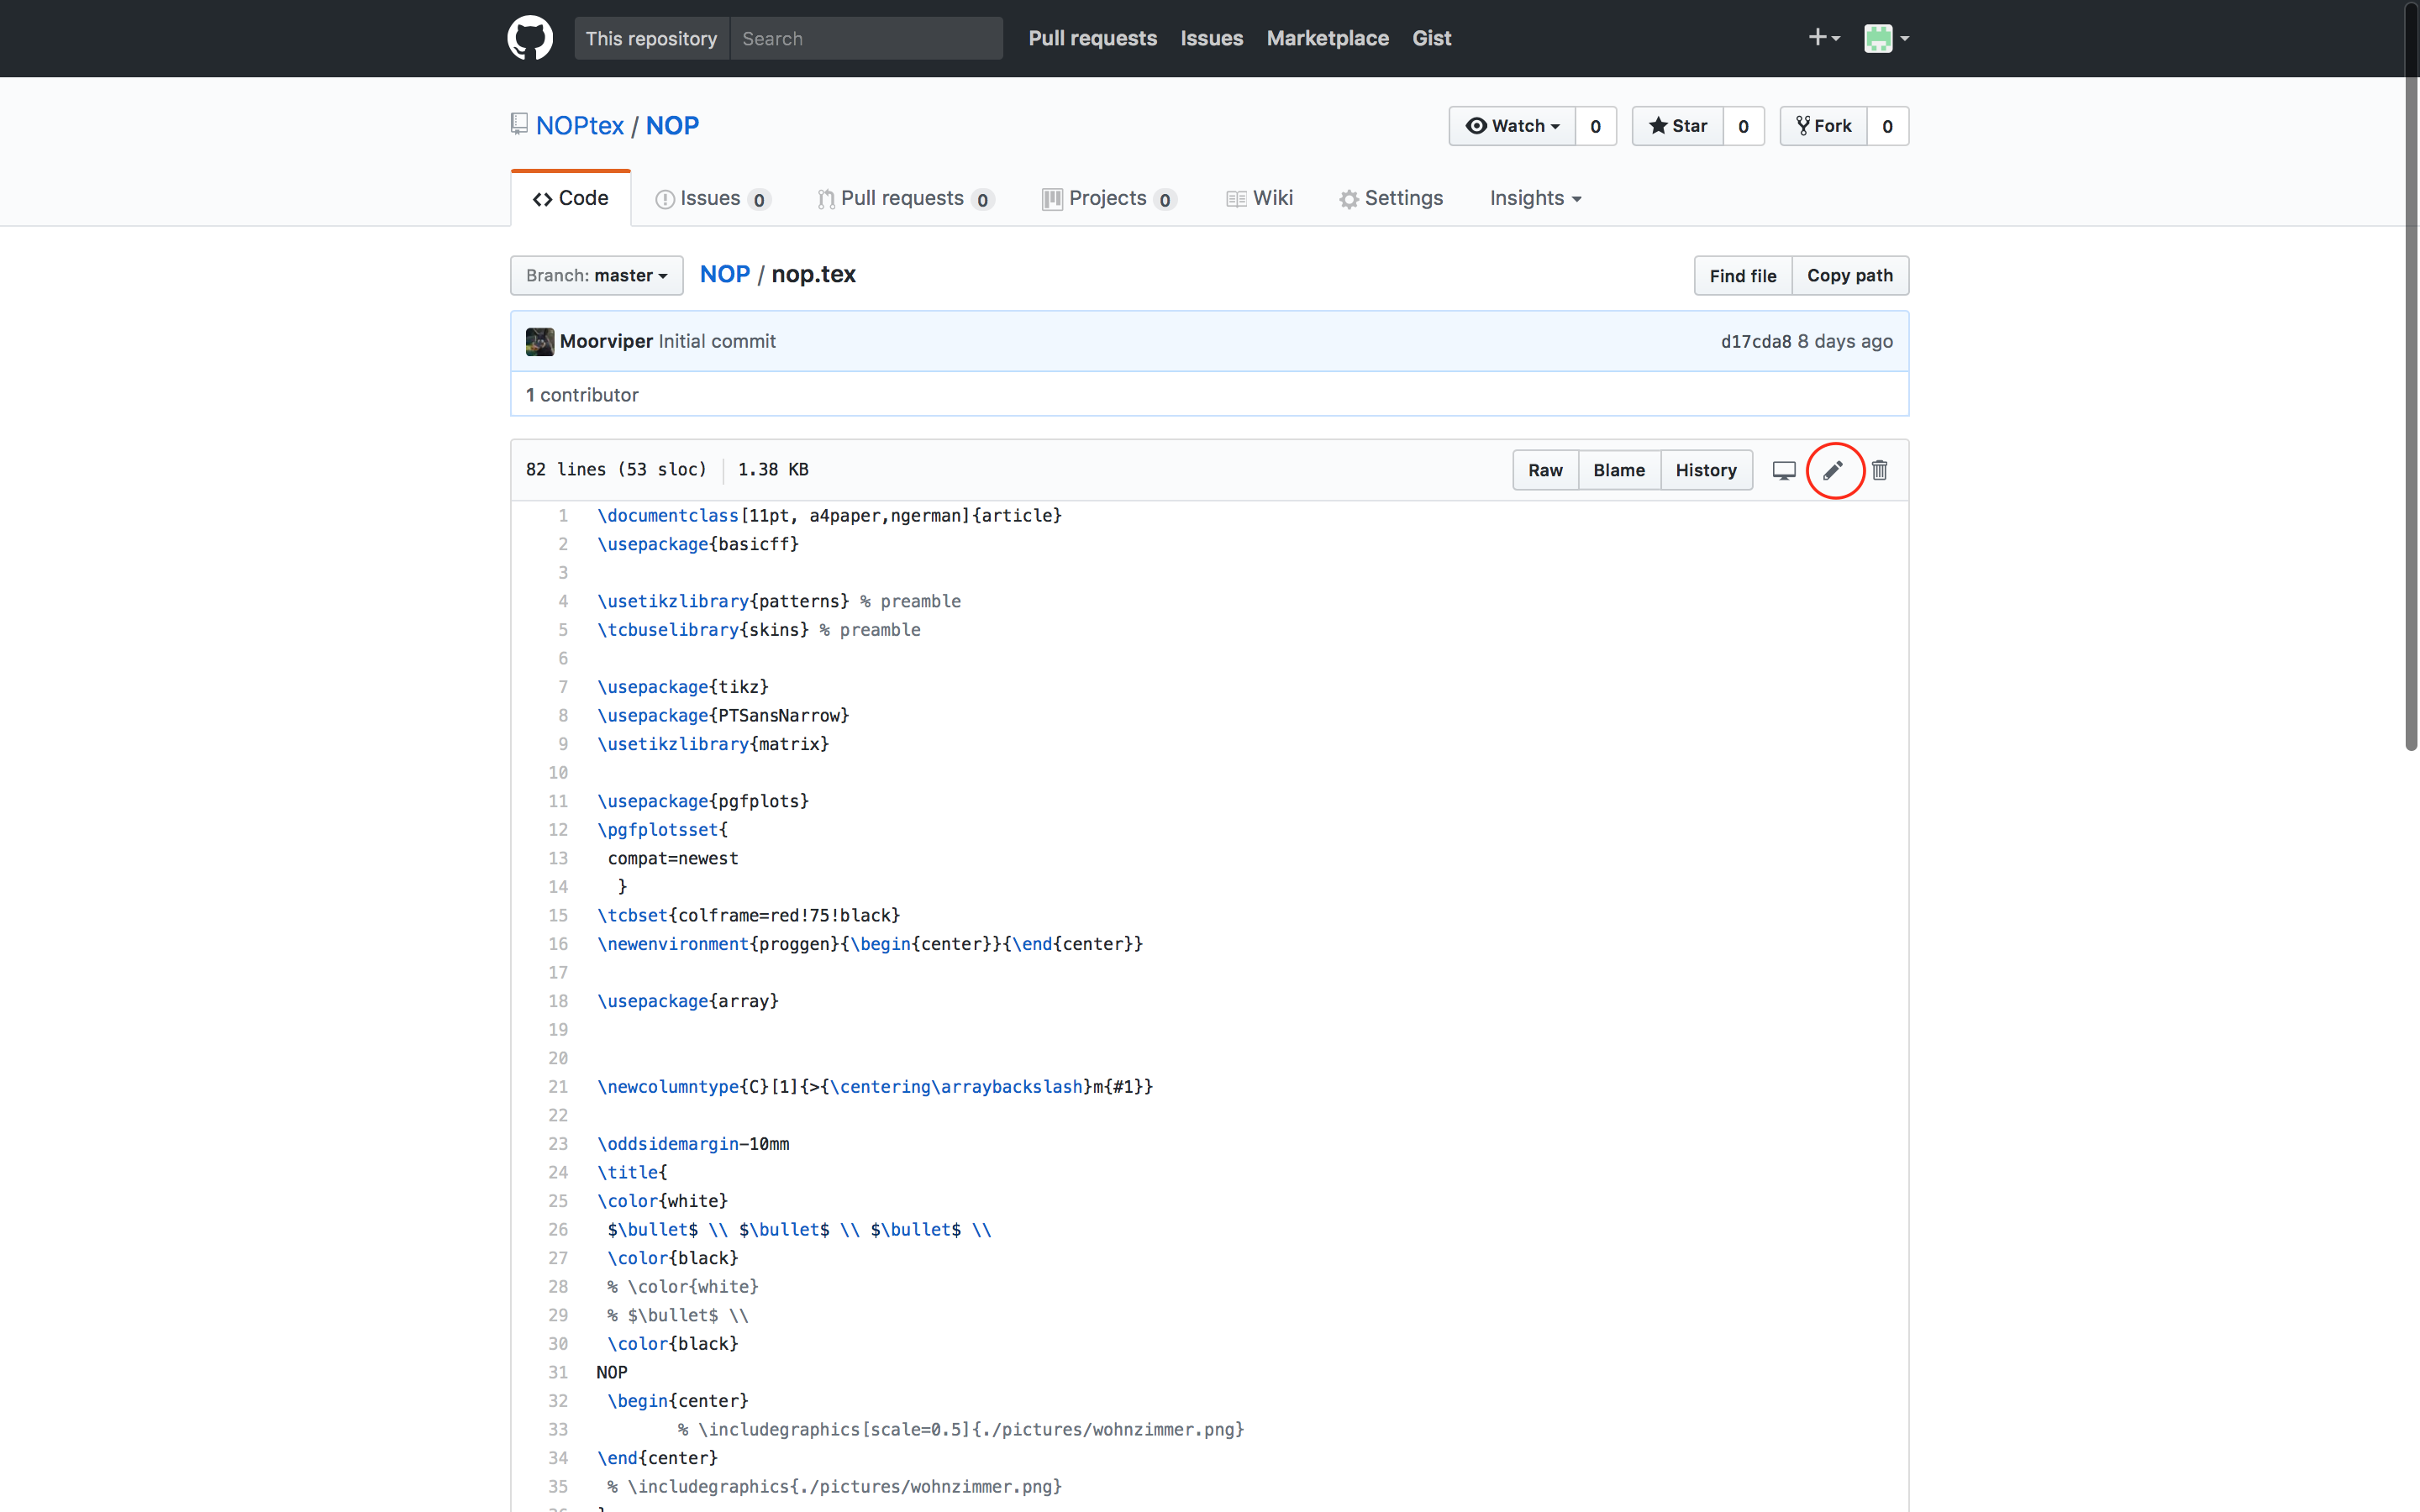
\includegraphics[width=1.0\textwidth]{./bilder/21edit.png}
\end{framed}

\end{minipage}}
% \hfill
\adjustbox{valign=t}{\begin{minipage}[t]{0.45\textwidth}
\vspace{0pt}
\huge
Man klickt auf den Stift zum editieren der Datei.
% \caption{Kapazität}
\end{minipage}}
% \end{figure}
% \vspace{0.5cm} % ----------------------------------- vspace
% \begin{figure}[ht]
\adjustbox{valign=t}{\begin{minipage}[t]{0.50\textwidth}
% \vspace{0.5cm}
\begin{framed}
  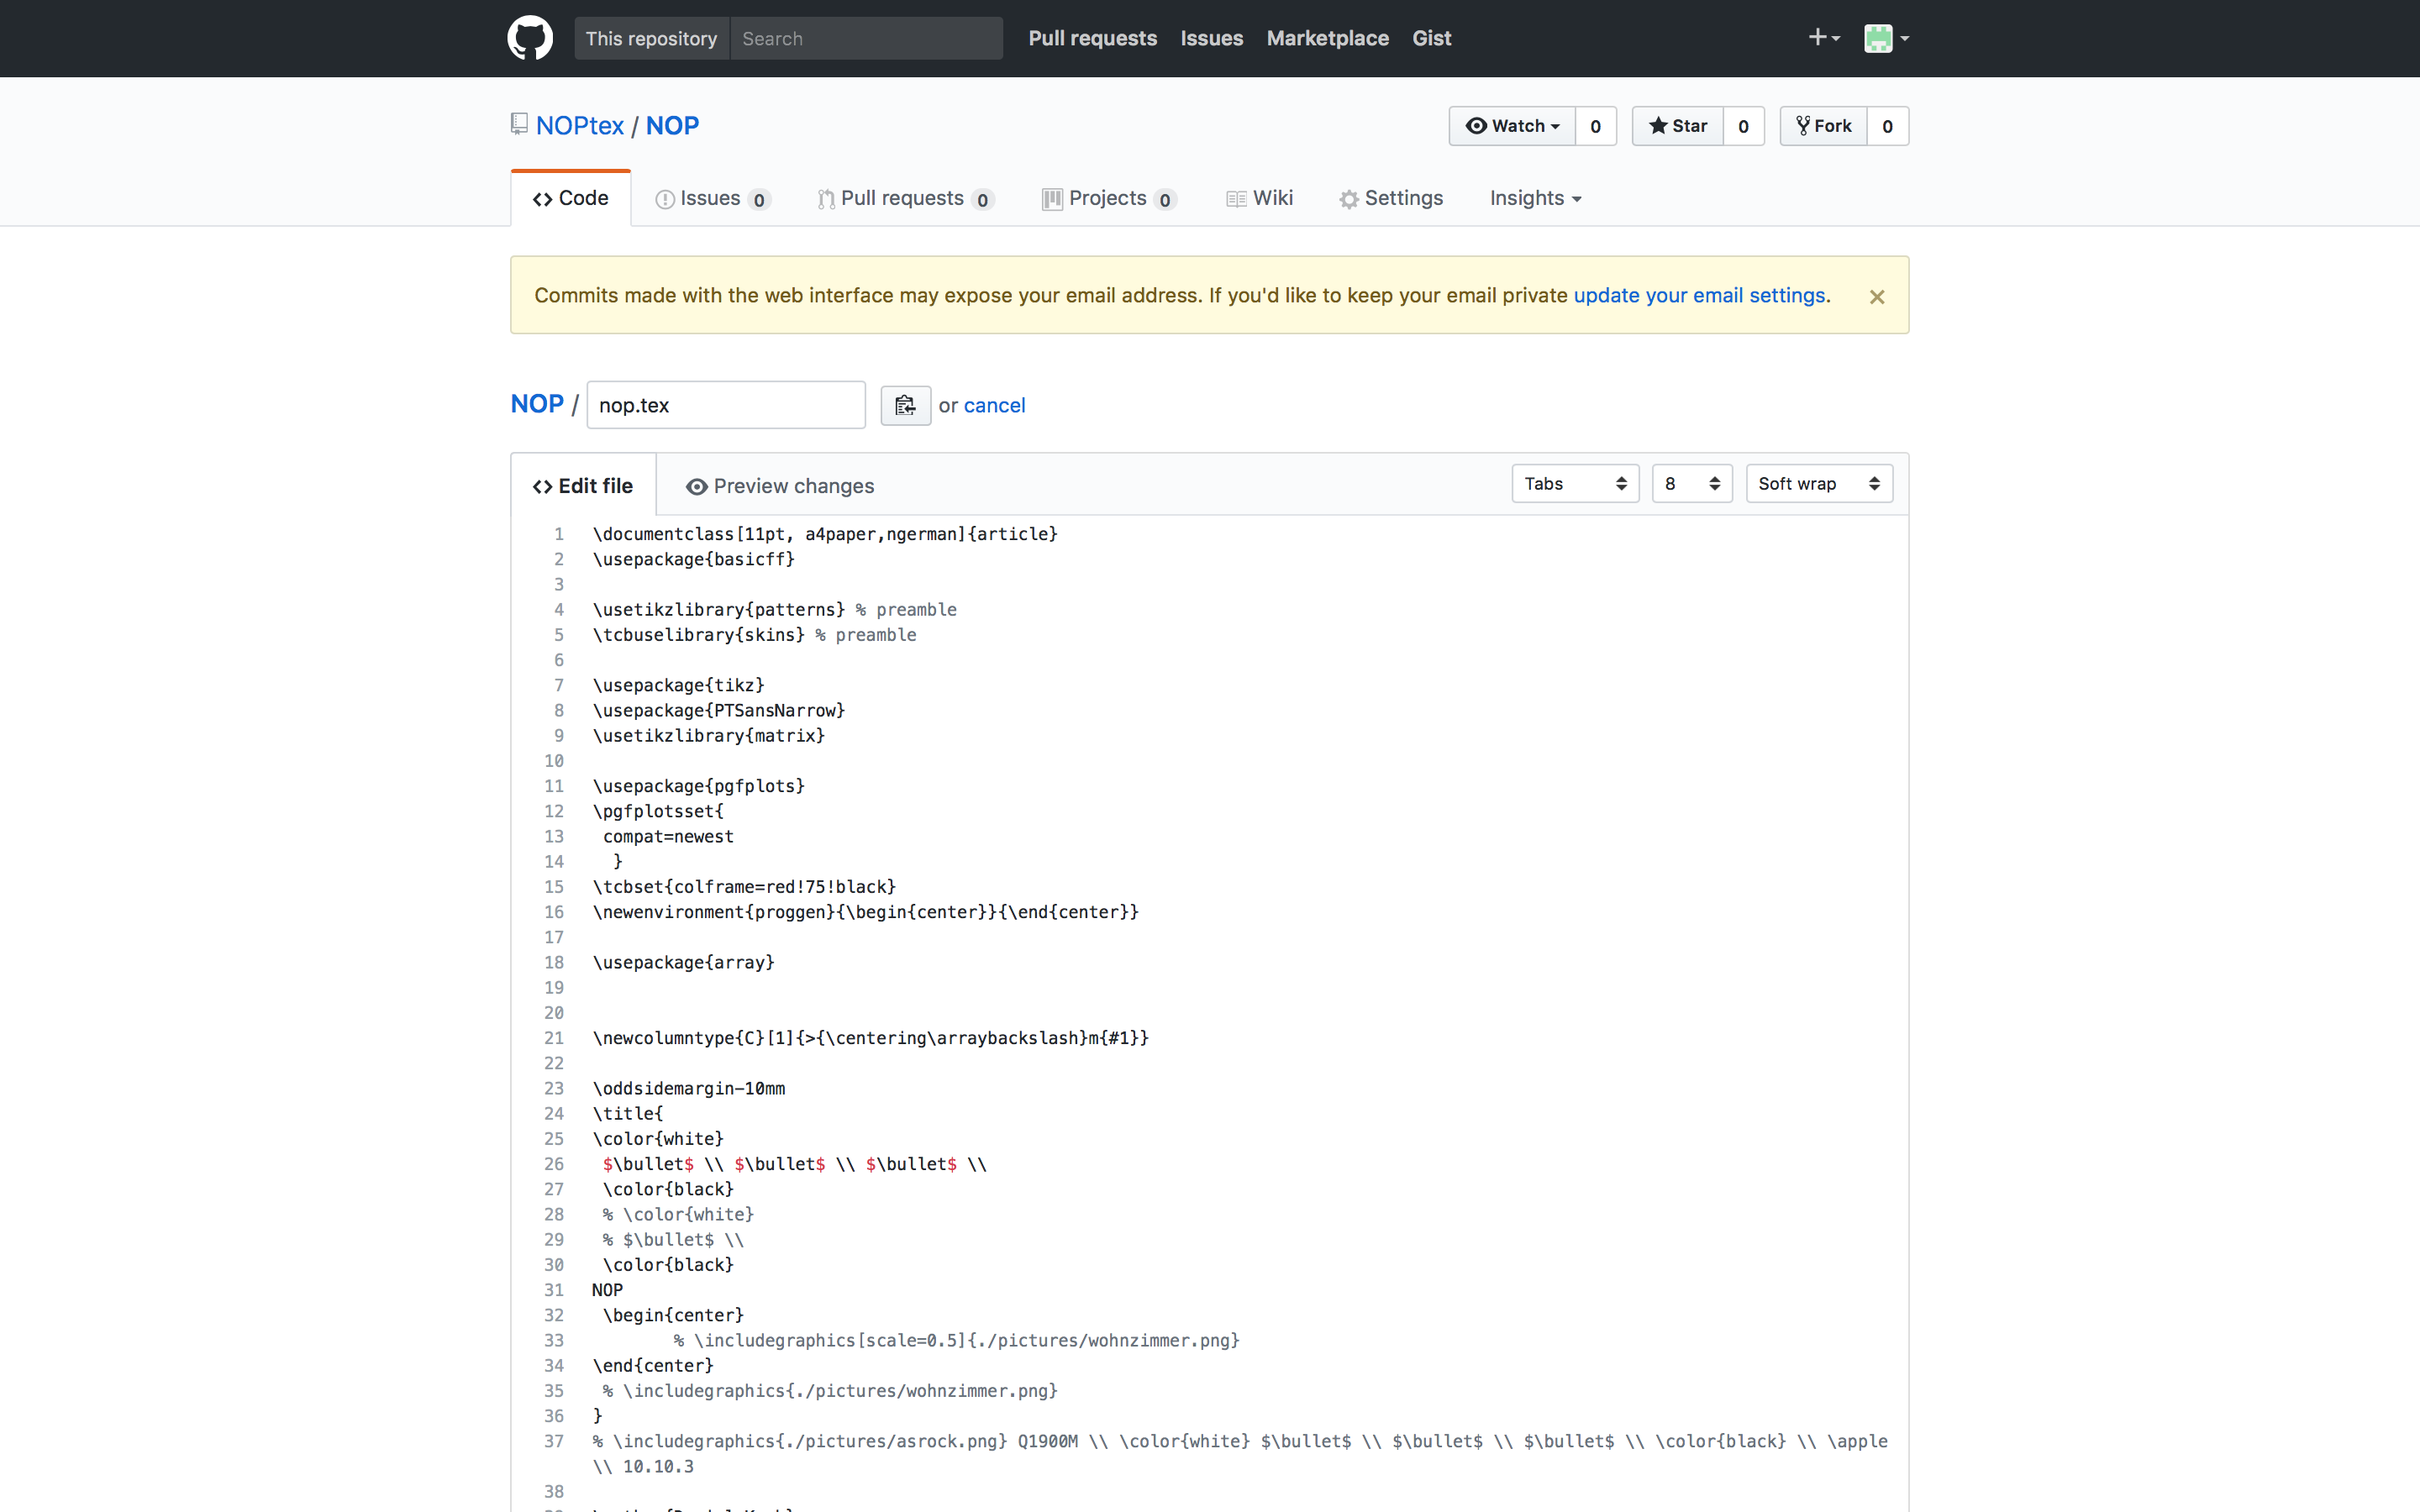
\includegraphics[width=1.0\textwidth]{./bilder/22edit.png}
\end{framed}

\end{minipage}}
\hfill
\adjustbox{valign=t}{\begin{minipage}[t]{0.45\textwidth}
\vspace{0pt}
\huge
Die Anzeige ändert sich geringfüging.
% \caption{Kapazität}
\end{minipage}}
\end{figure}

\clearpage % GleitObjekte anzeigen

\newpage % ============================================= Newpage ===================


\begin{figure}[ht]
  % \section{Release mit Tag erstellen und bauen}
\adjustbox{valign=t}{\begin{minipage}[t]{0.50\textwidth}
\begin{framed}
  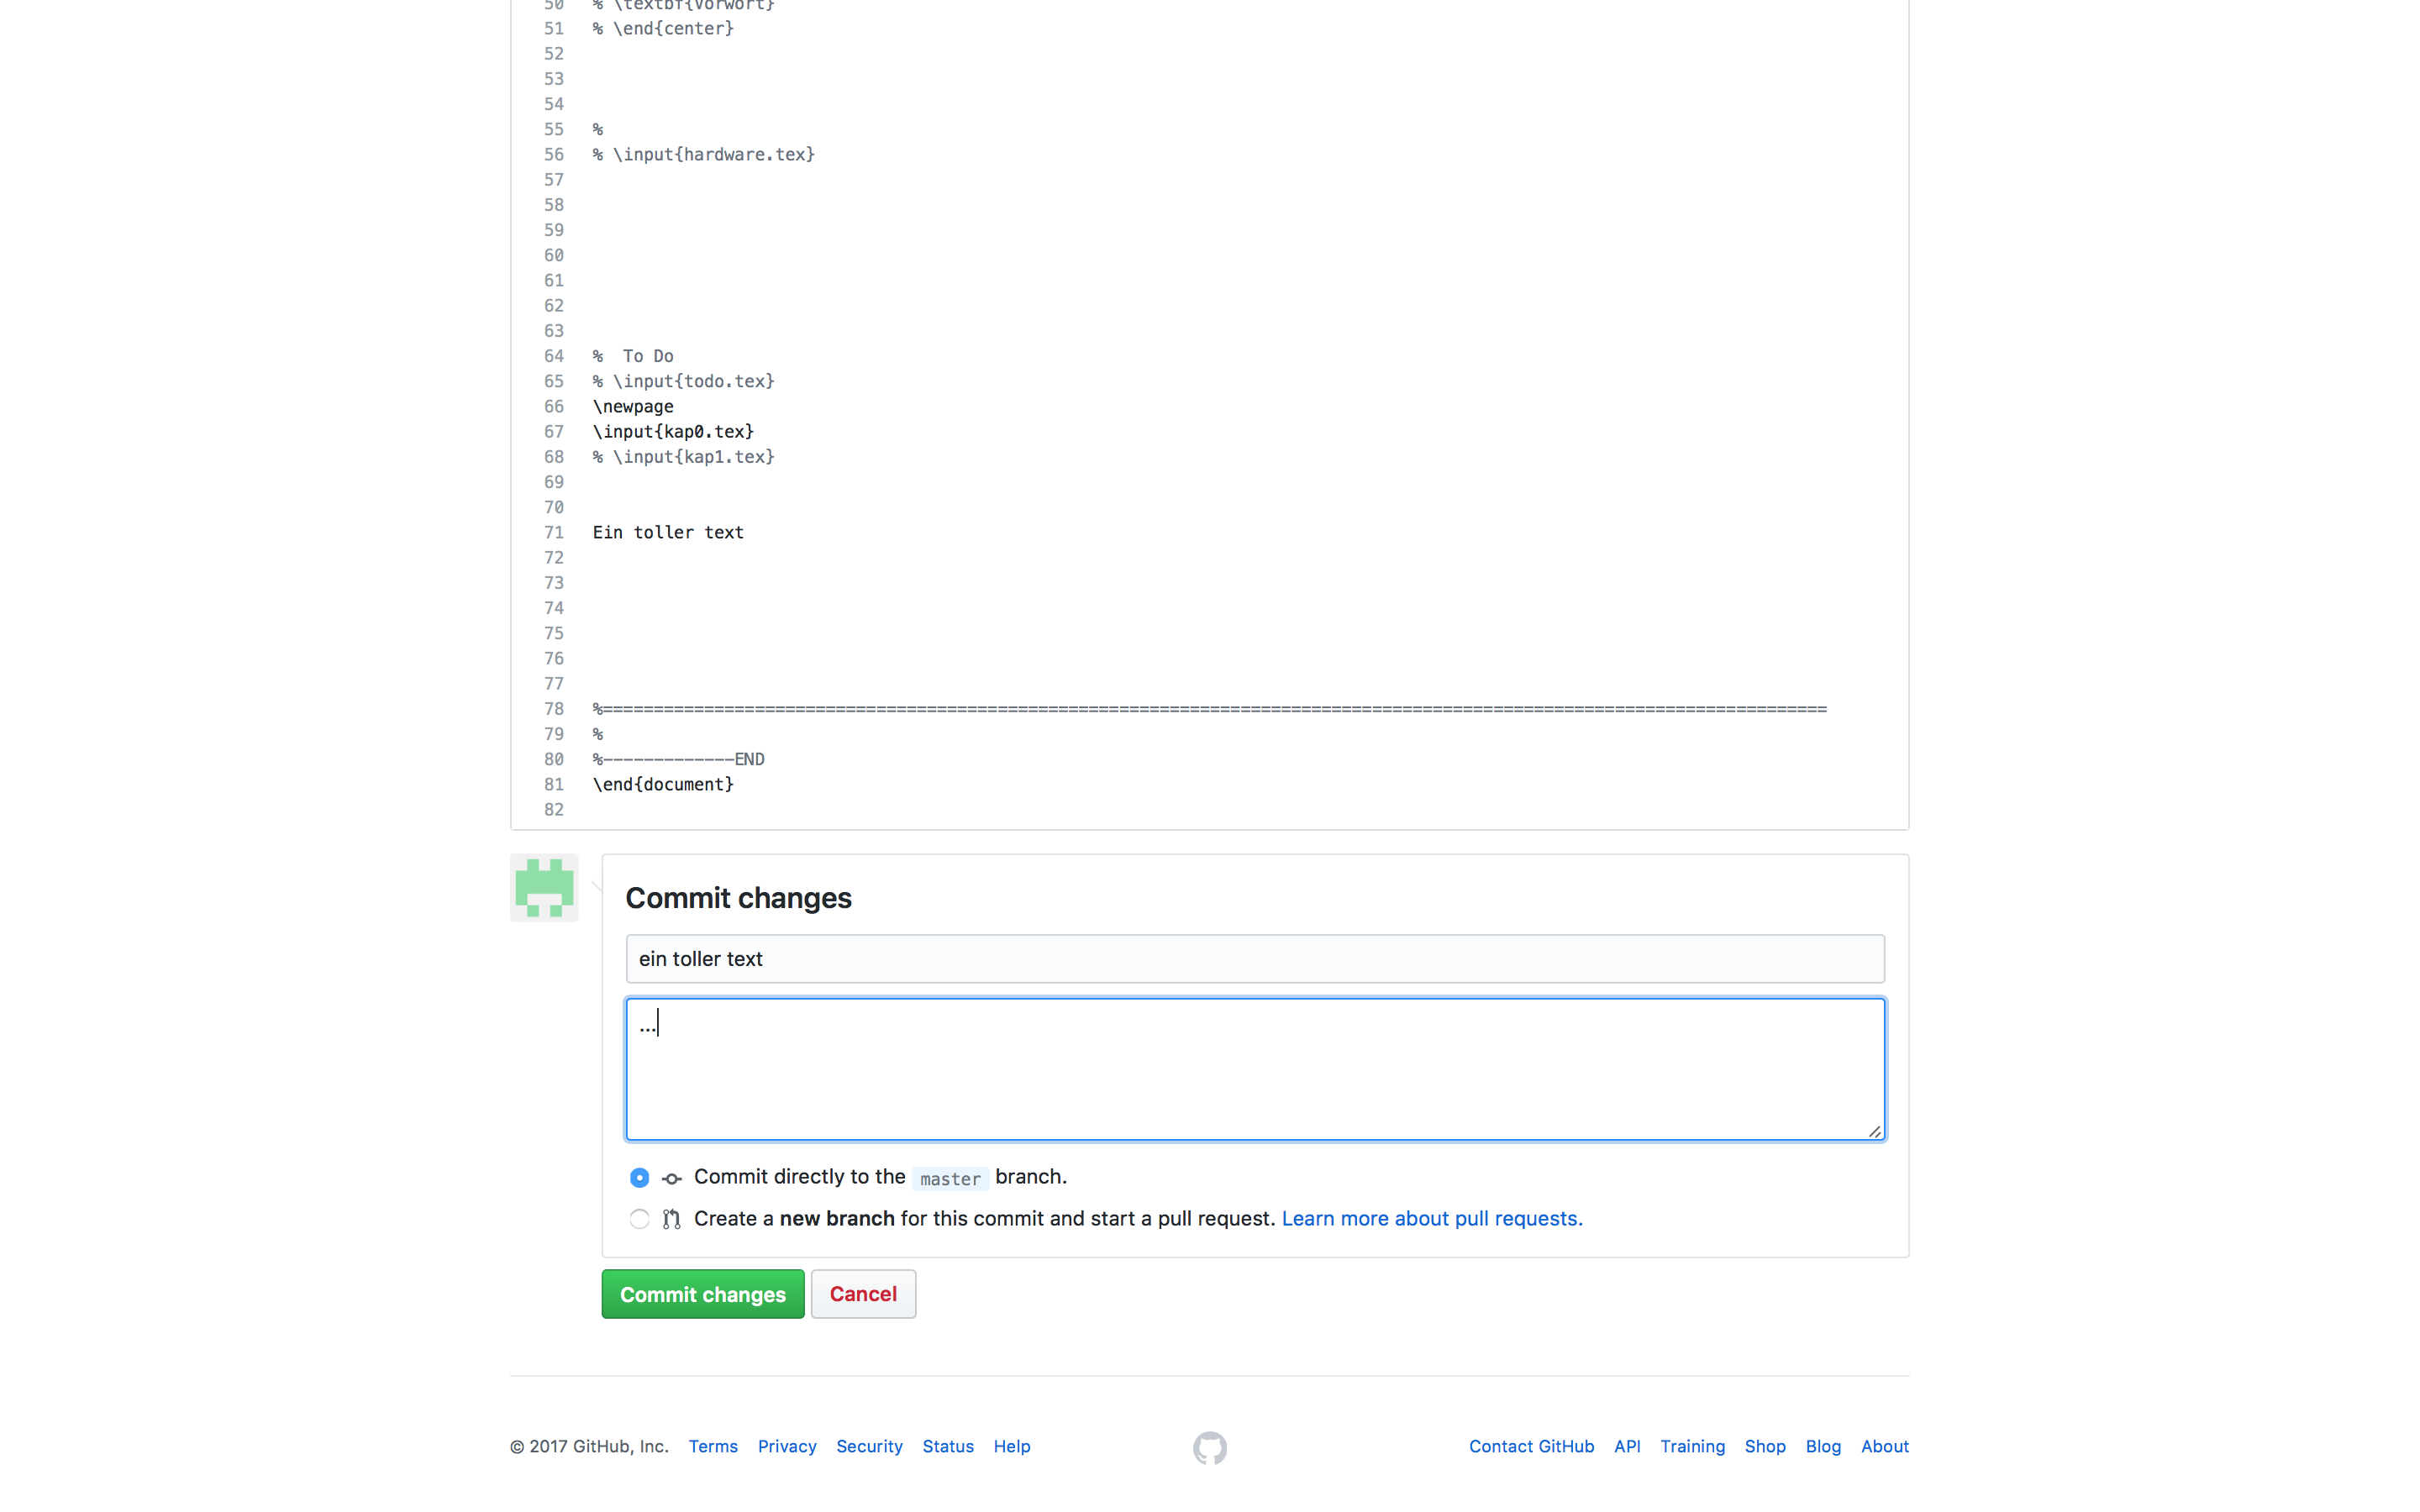
\includegraphics[width=1.0\textwidth]{./bilder/23createRelease.png}
\end{framed}

\end{minipage}}
% \hfill
\adjustbox{valign=t}{\begin{minipage}[t]{0.45\textwidth}
\vspace{0pt}
\huge
Text, Titel und Beschreibung hinzufügen.
% \caption{Kapazität}
\end{minipage}}
% \end{figure}
% \vspace{0.5cm} % ----------------------------------- vspace
% \begin{figure}[ht]
\adjustbox{valign=t}{\begin{minipage}[t]{0.50\textwidth}
% \vspace{0.5cm}
\begin{framed}
  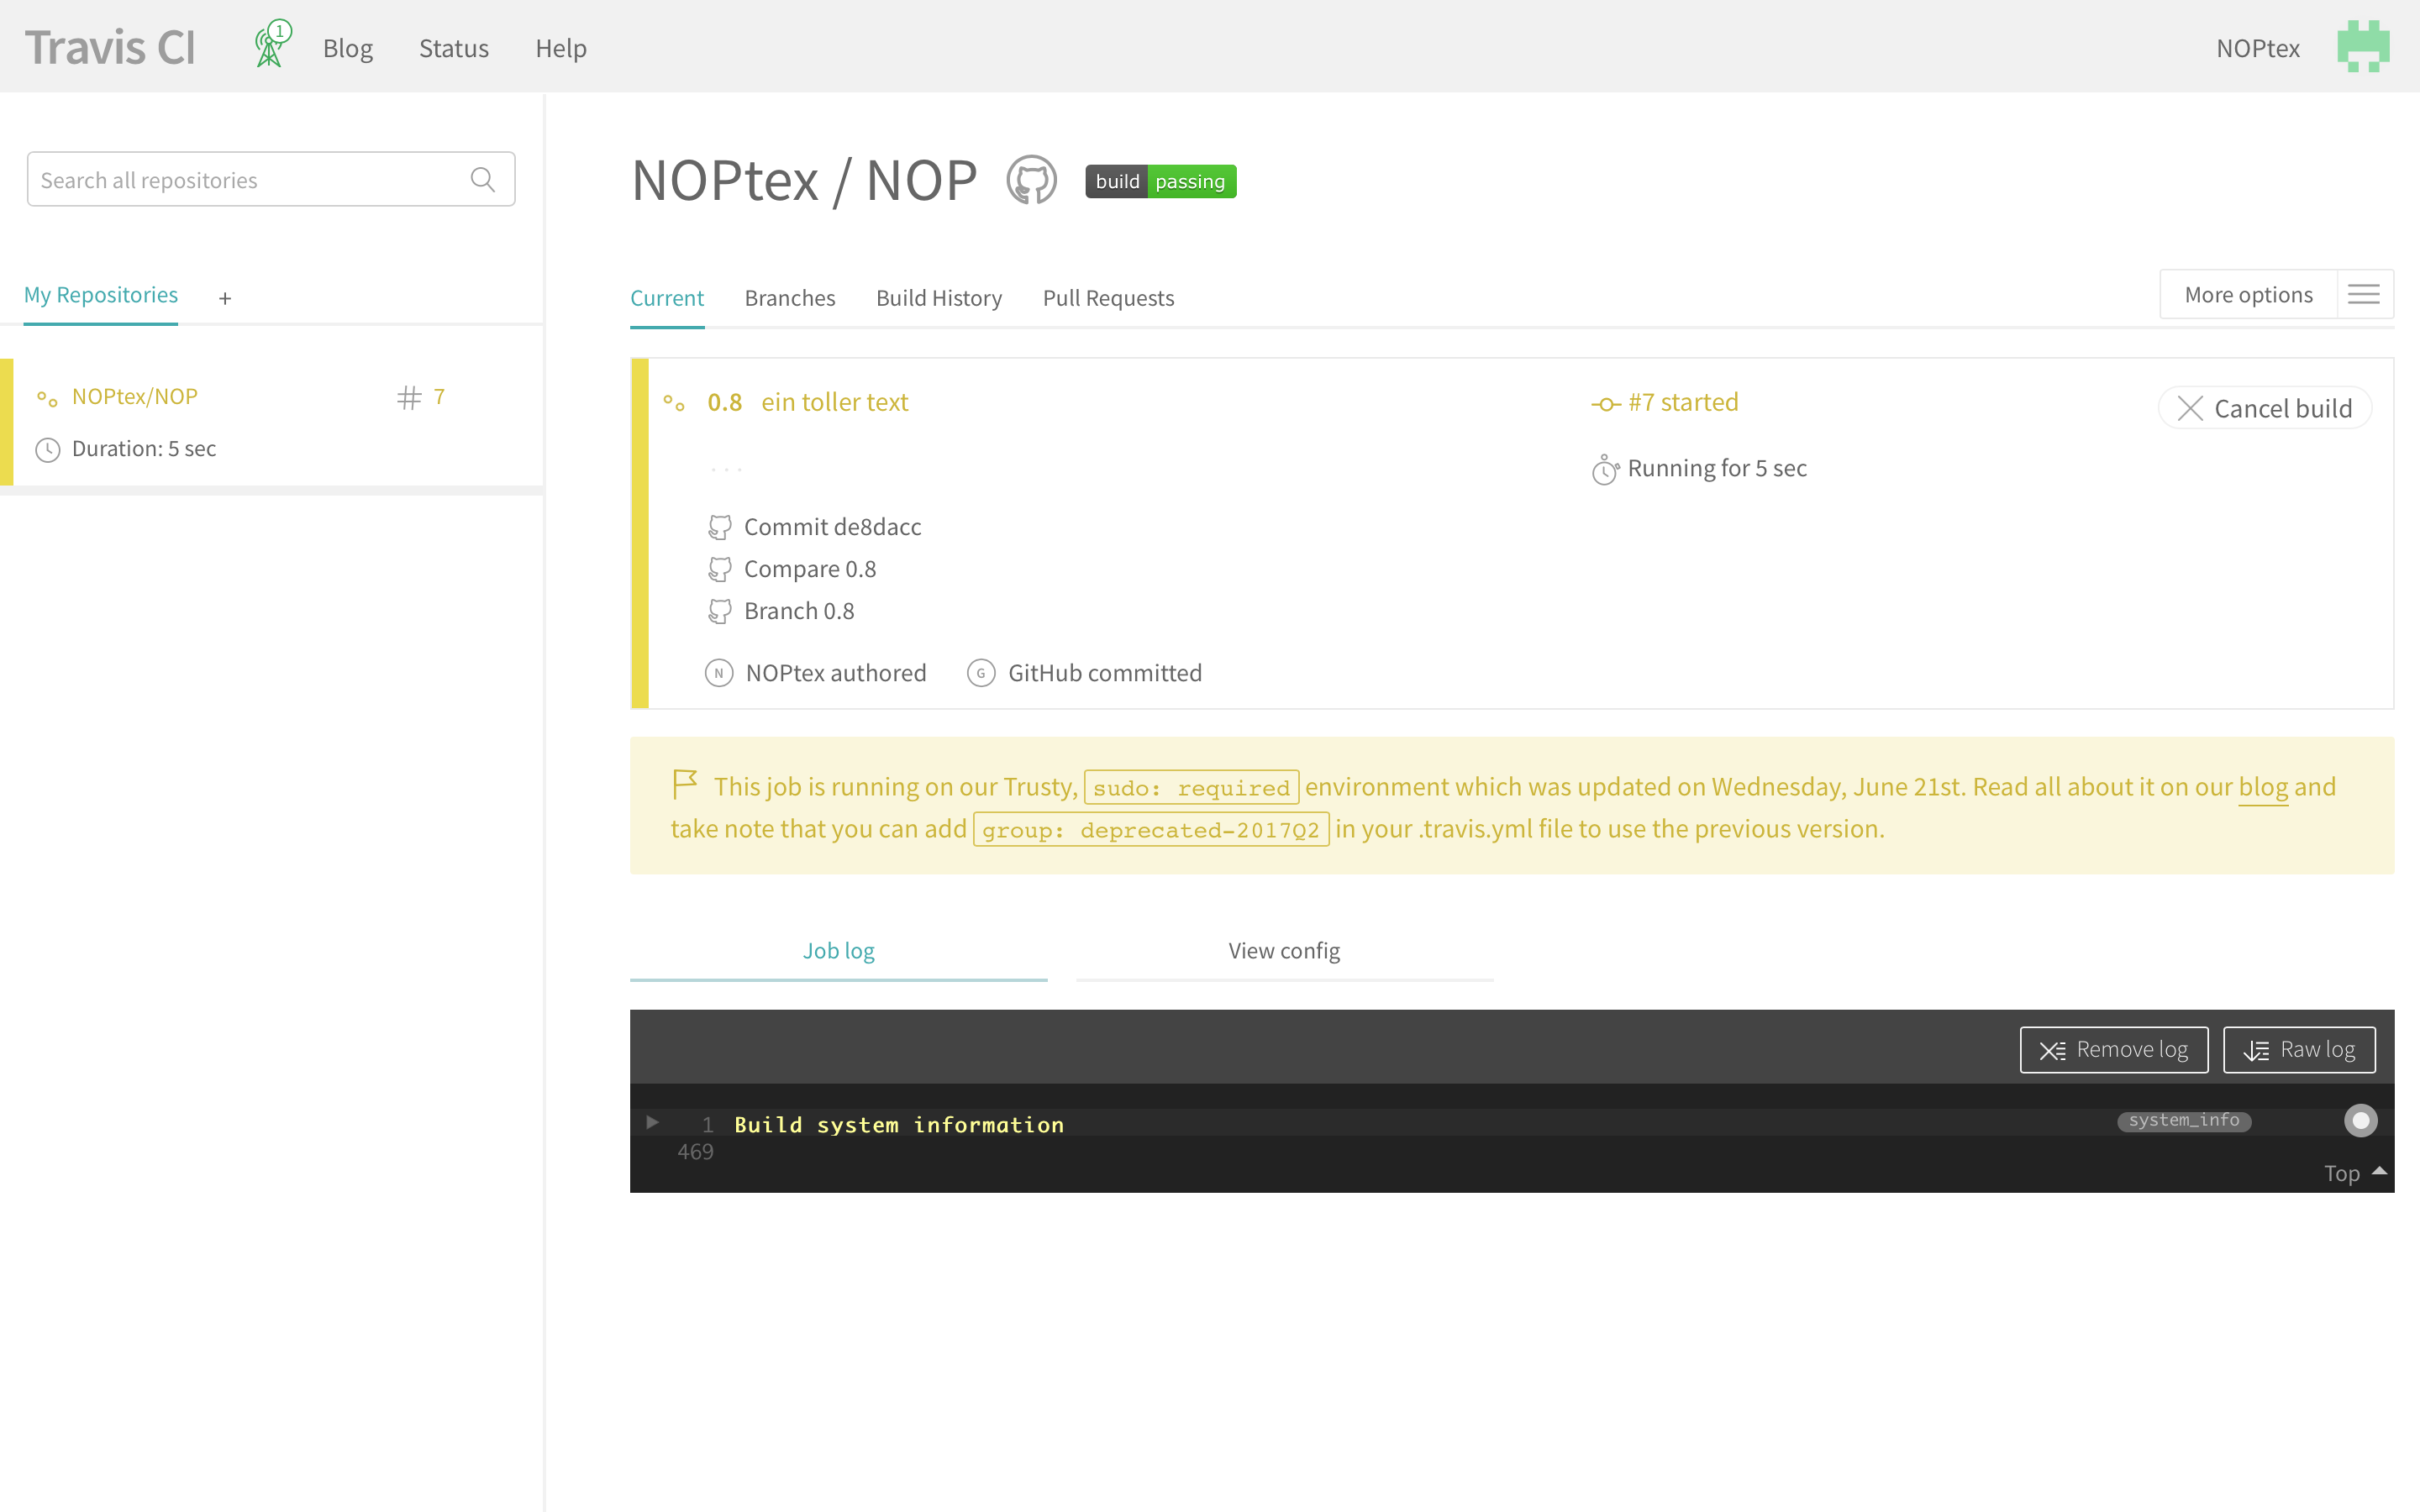
\includegraphics[width=1.0\textwidth]{./bilder/24baut.png}
\end{framed}

\end{minipage}}
\hfill
\adjustbox{valign=t}{\begin{minipage}[t]{0.45\textwidth}
\vspace{0pt}
\huge
Kontrolle bei Travis und es baut.\\
(Das dauert dann so 7-8 Minuten.)
% \caption{Kapazität}
\end{minipage}}
\end{figure}

\clearpage % GleitObjekte anzeigen


\newpage % ============================================= Newpage ===================


\begin{figure}[ht]
  \section{Erfolgreich gebaut}
\adjustbox{valign=t}{\begin{minipage}[t]{0.50\textwidth}
\begin{framed}
  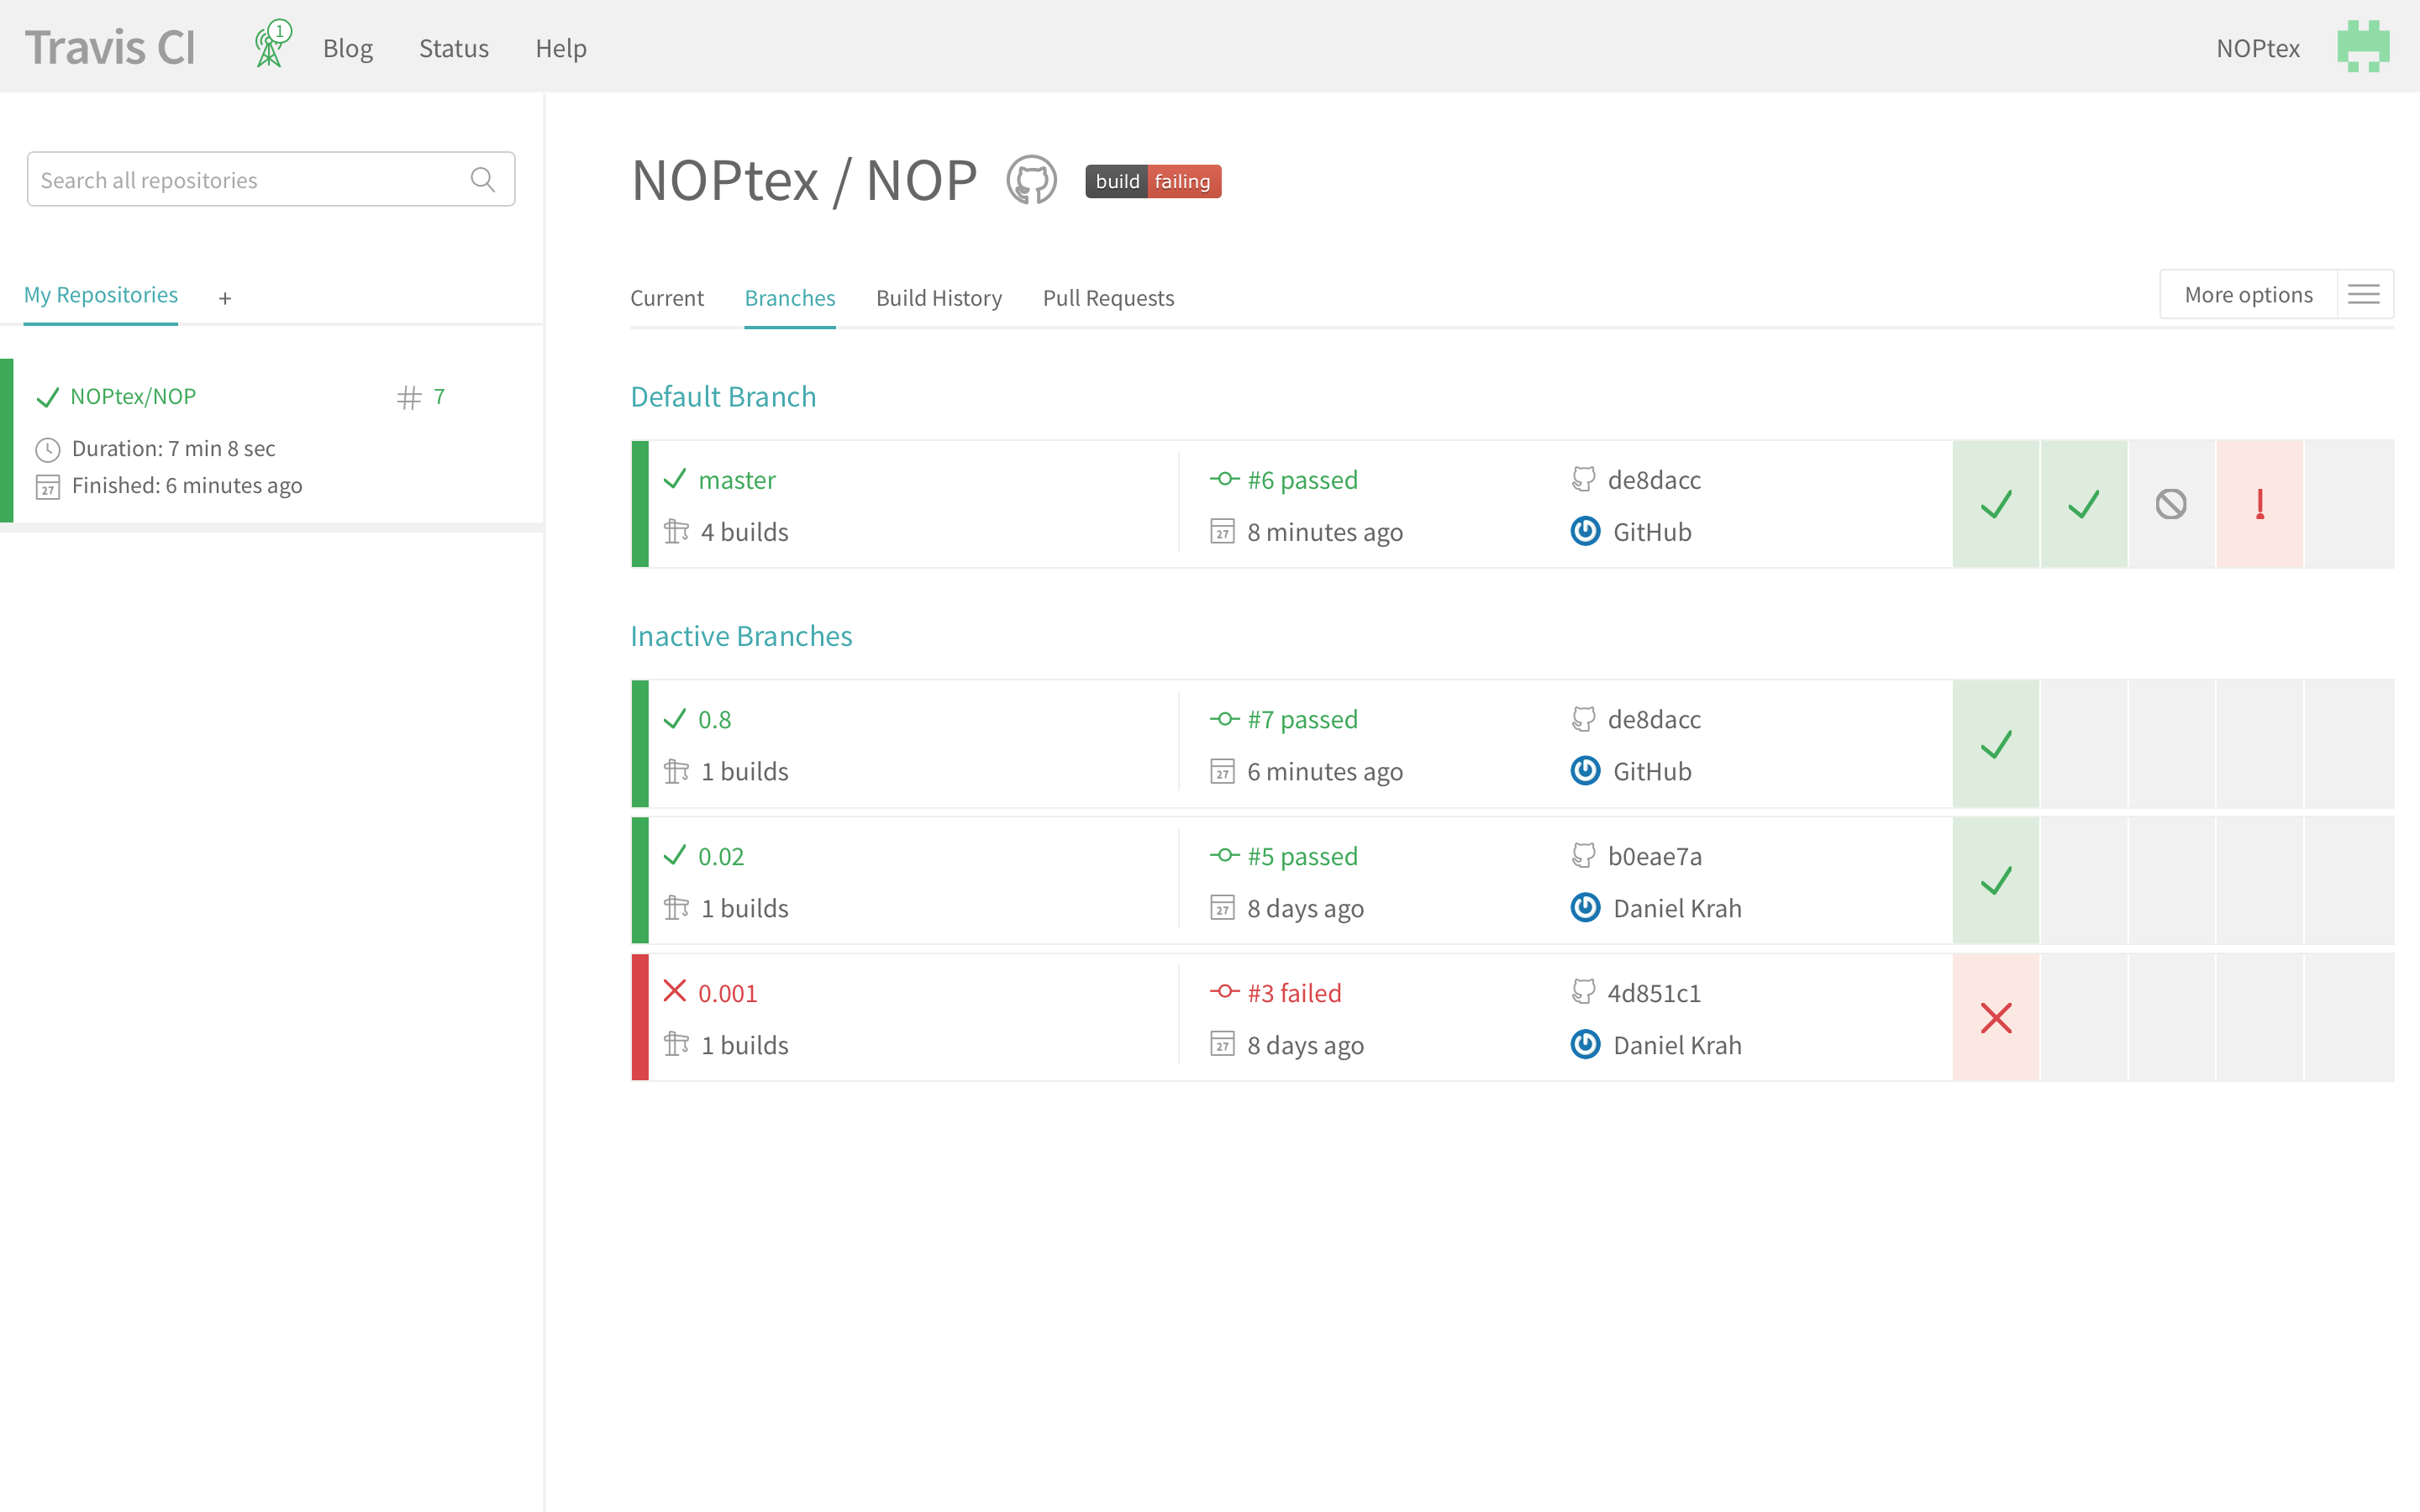
\includegraphics[width=1.0\textwidth]{./bilder/25gebaut.png}
\end{framed}

\end{minipage}}
% \hfill
\adjustbox{valign=t}{\begin{minipage}[t]{0.45\textwidth}
\vspace{0pt}
\huge
Wenn fertig sieht es so aus.
% \caption{Kapazität}
\end{minipage}}
% \end{figure}
% \vspace{0.5cm} % ----------------------------------- vspace
% \begin{figure}[ht]
\adjustbox{valign=t}{\begin{minipage}[t]{0.50\textwidth}
% \vspace{0.5cm}
\begin{framed}
  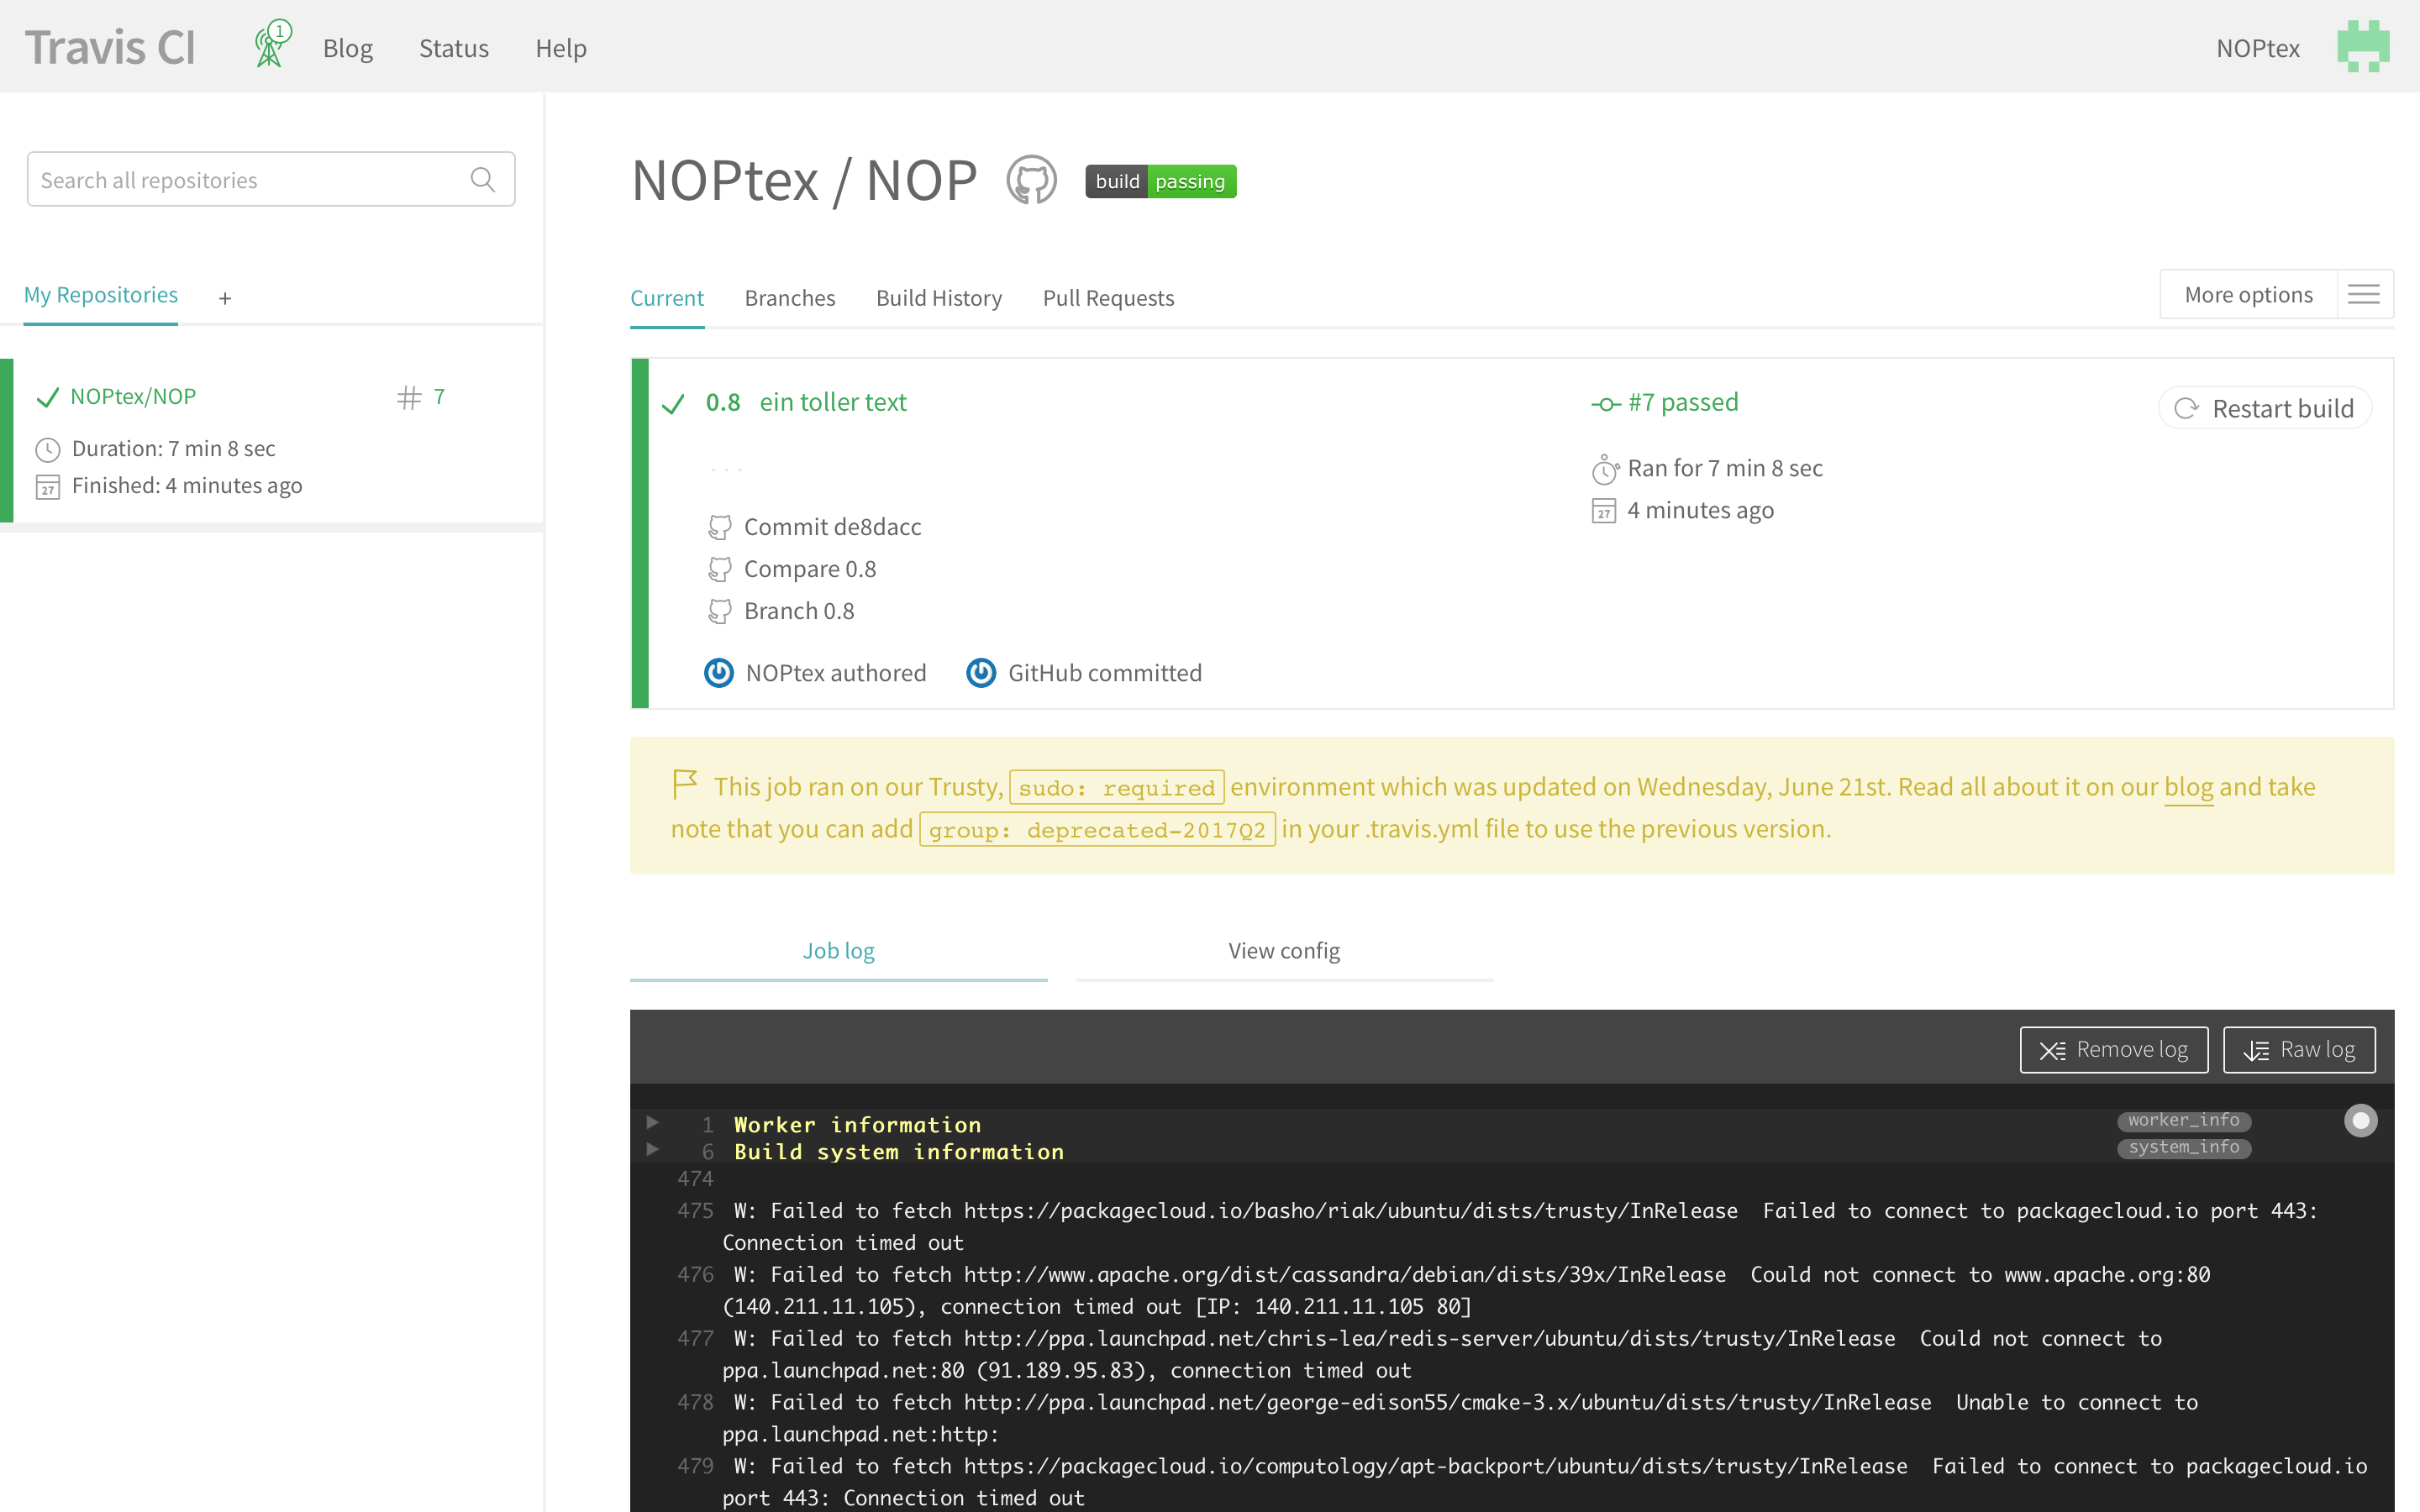
\includegraphics[width=1.0\textwidth]{./bilder/26details.png}
\end{framed}

\end{minipage}}
\hfill
\adjustbox{valign=t}{\begin{minipage}[t]{0.45\textwidth}
\vspace{0pt}
\huge
Optional kann man die Log-Ausgaben anschauen. \\
Aber in diesem Fall ging ja alles gut.
% \caption{Kapazität}
\end{minipage}}
\end{figure}

\clearpage % GleitObjekte anzeigen

\newpage % ============================================= Newpage ===================


\begin{figure}[ht]
  \section{Github kontrollieren und PDF überprüfen}
\adjustbox{valign=t}{\begin{minipage}[t]{0.50\textwidth}
\begin{framed}
  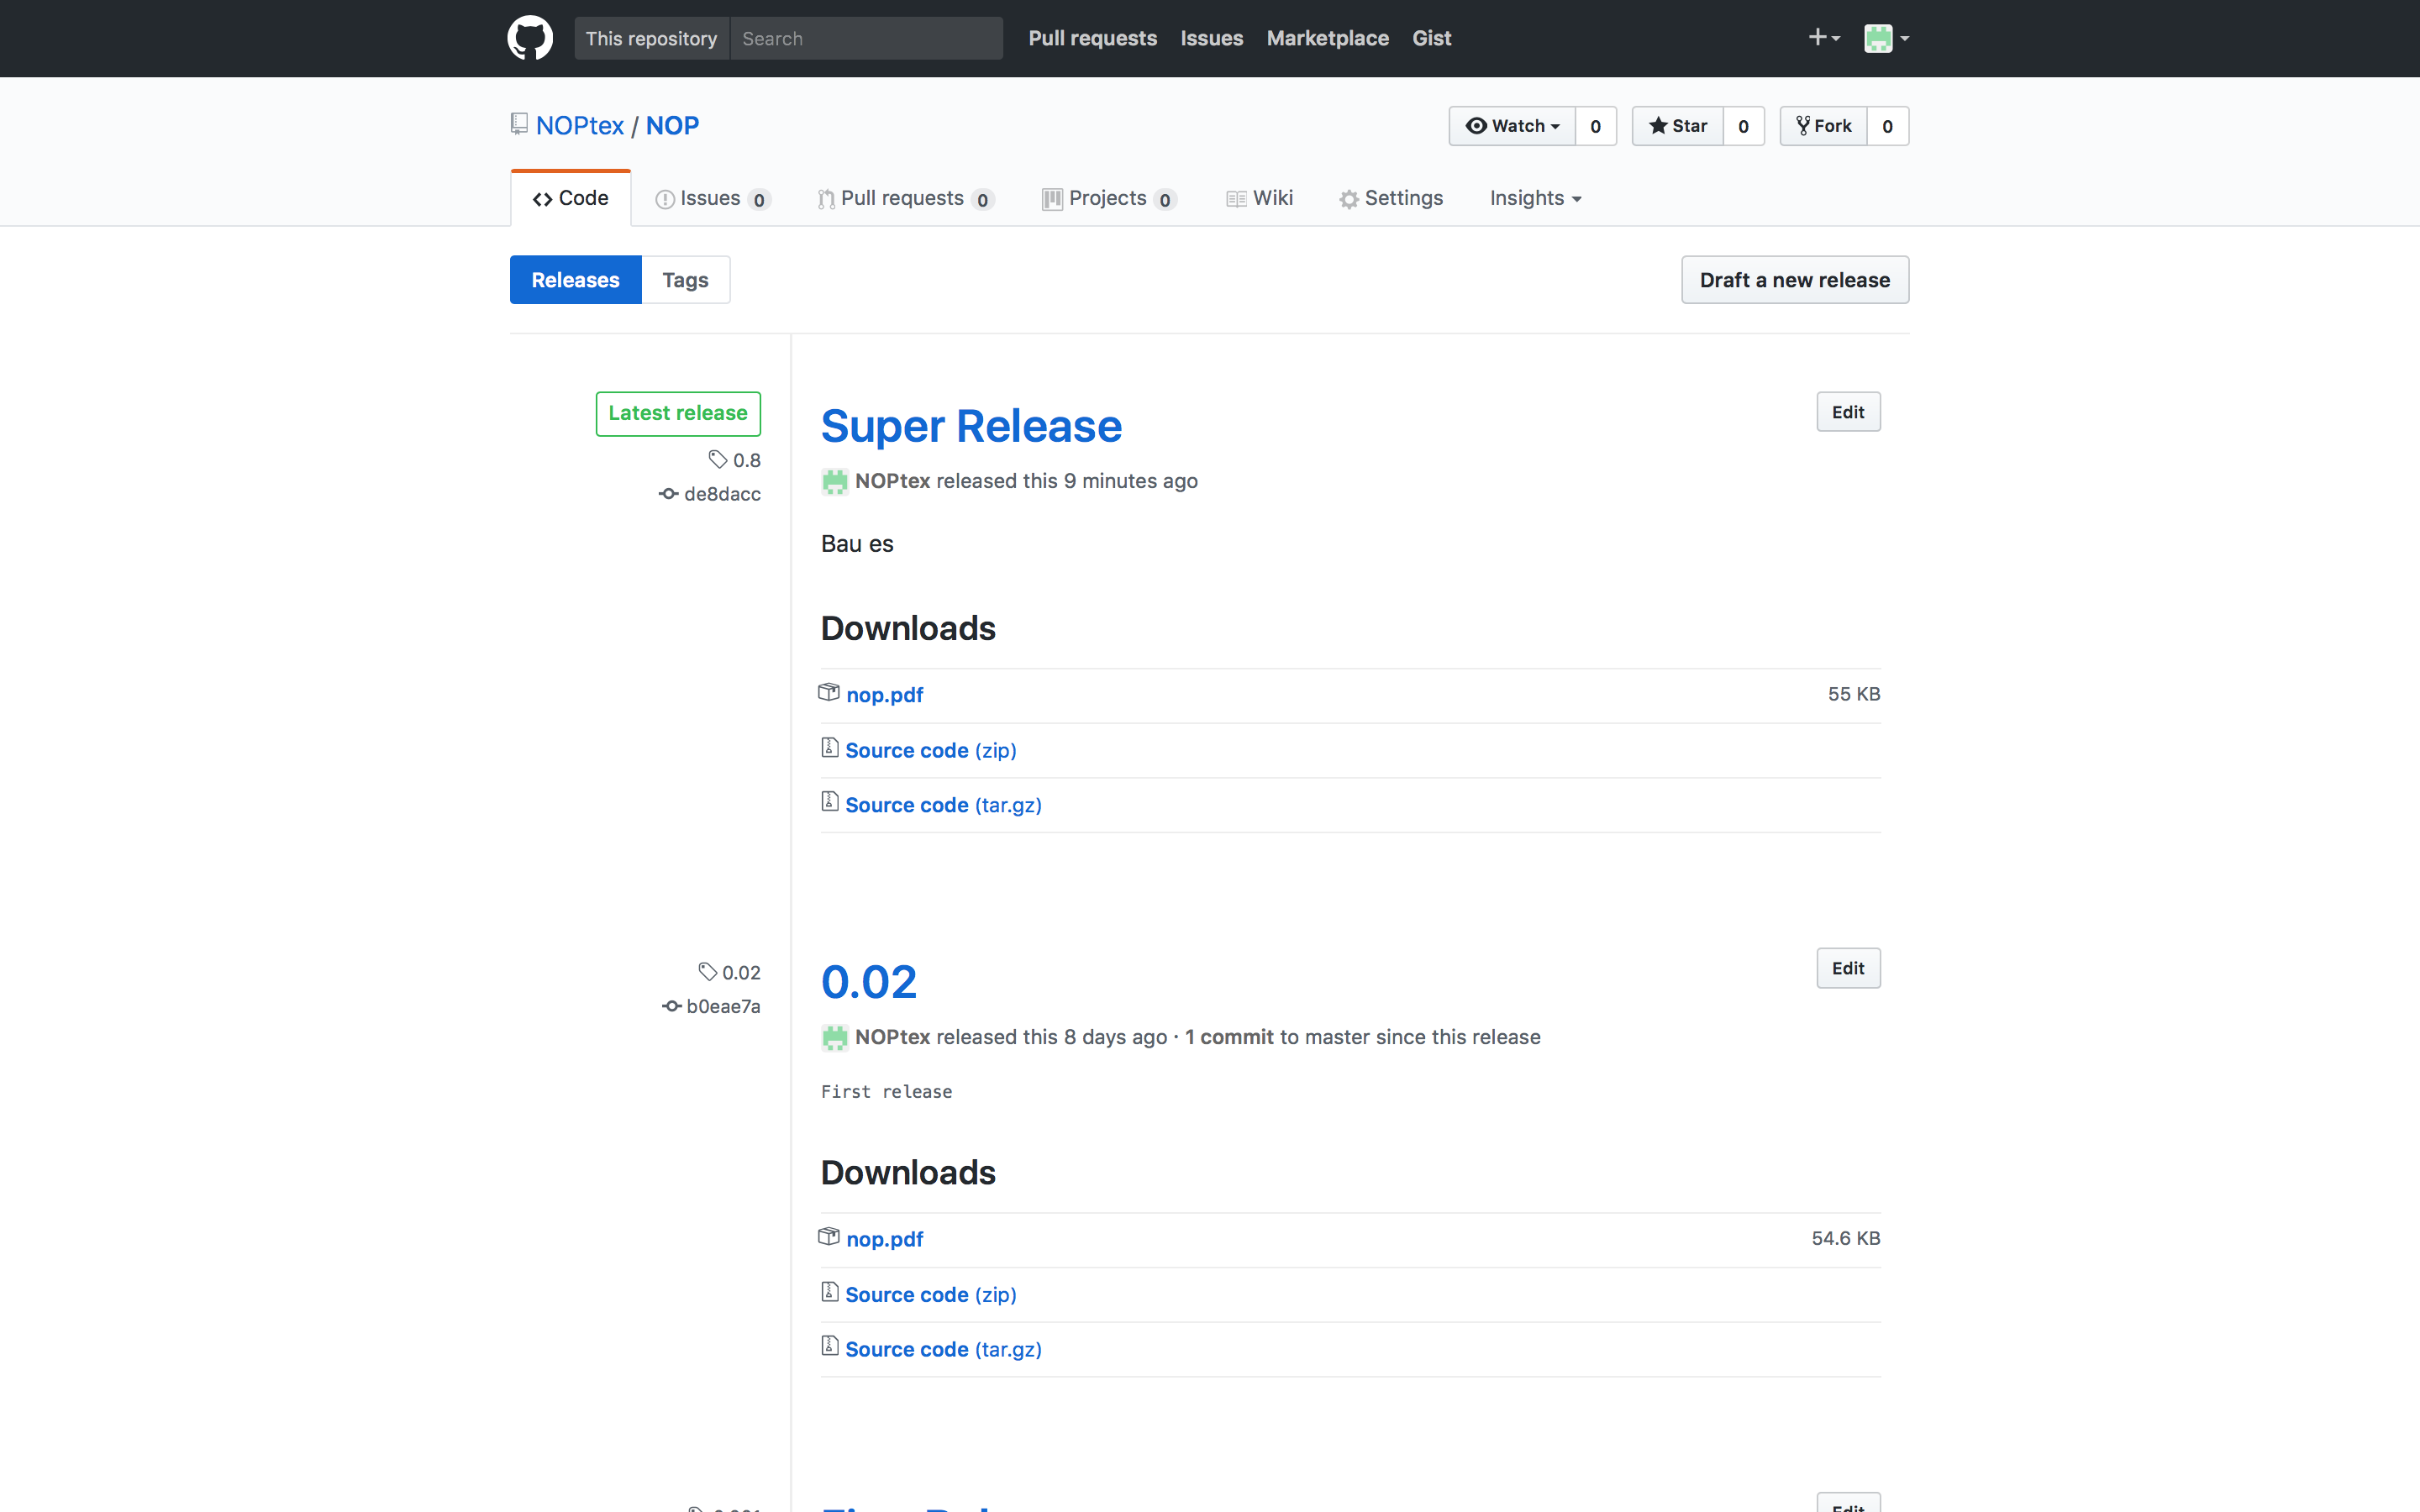
\includegraphics[width=1.0\textwidth]{./bilder/27release.png}
\end{framed}

\end{minipage}}
% \hfill
\adjustbox{valign=t}{\begin{minipage}[t]{0.45\textwidth}
\vspace{0pt}
\huge
Auf GitHub ist nun auch die PDF under Releases ...
% \caption{Kapazität}
\end{minipage}}
% \end{figure}
% \vspace{0.5cm} % ----------------------------------- vspace
% \begin{figure}[ht]
\adjustbox{valign=t}{\begin{minipage}[t]{0.50\textwidth}
% \vspace{0.5cm}
\begin{framed}
  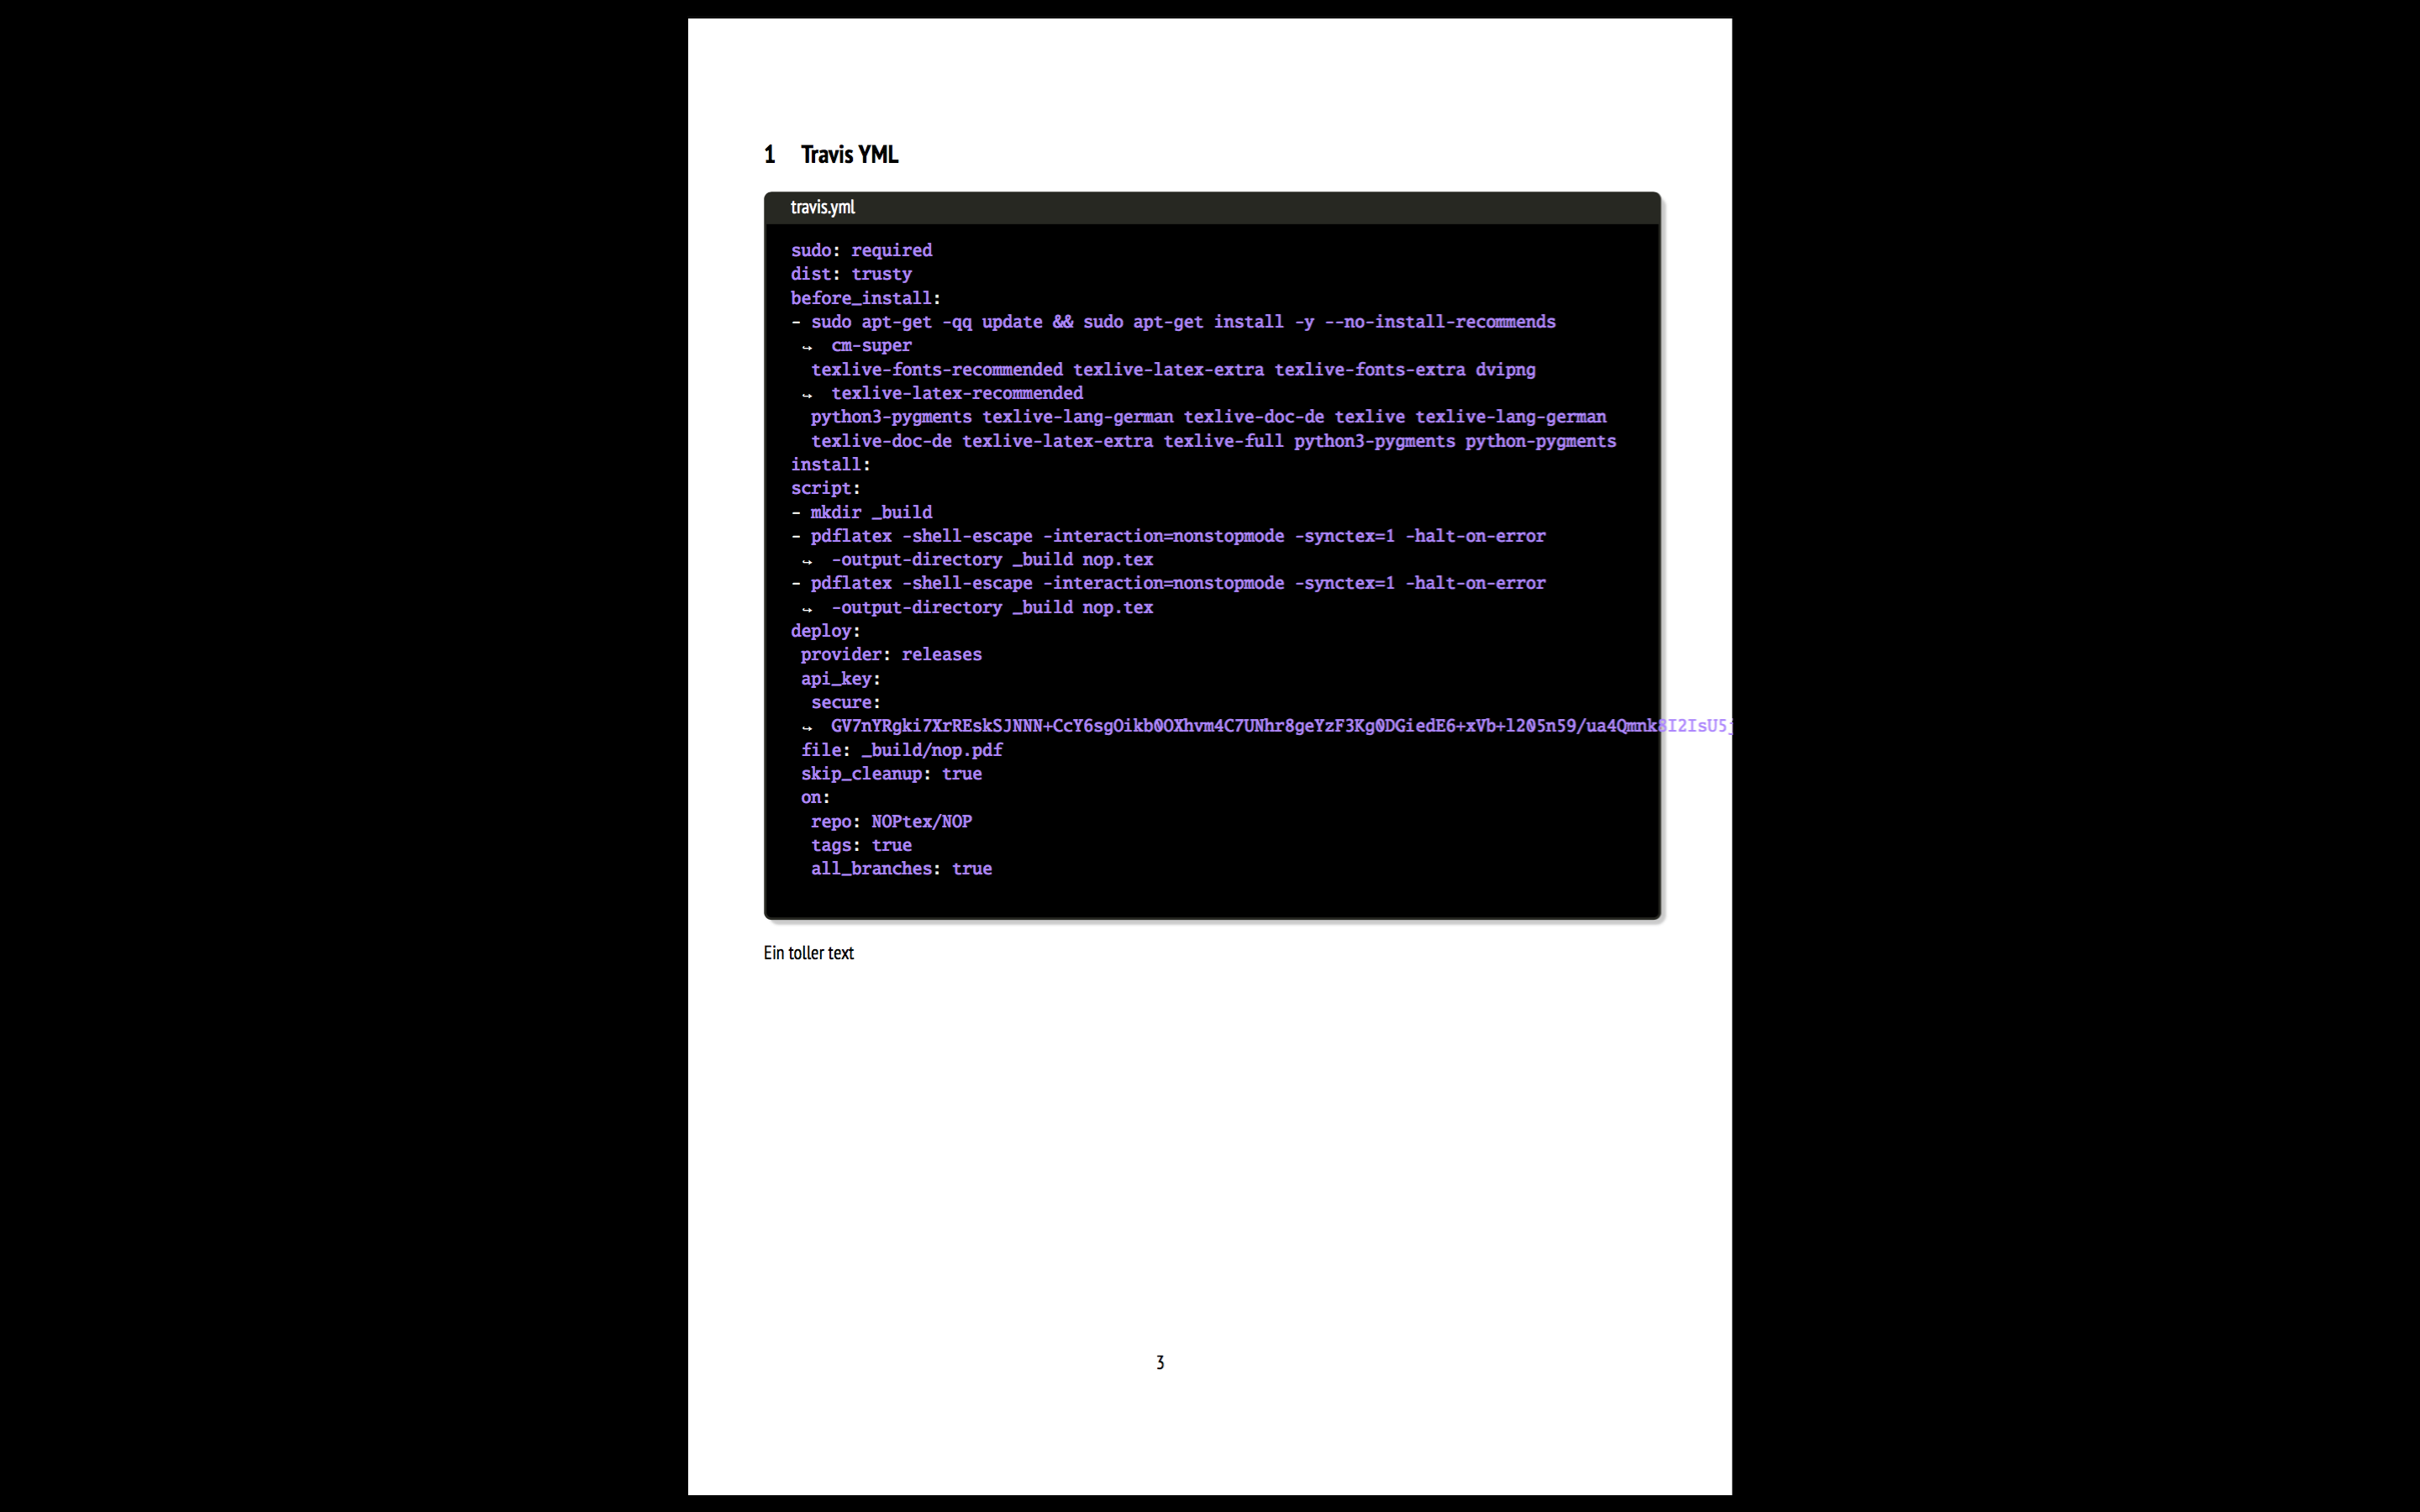
\includegraphics[width=1.0\textwidth]{./bilder/28fertig.png}
\end{framed}

\end{minipage}}
\hfill
\adjustbox{valign=t}{\begin{minipage}[t]{0.45\textwidth}
\vspace{0pt}
\huge
PDF sieht gut aus und die Änderung ist mit drinnen.
% \caption{Kapazität}
\end{minipage}}
\end{figure}

\clearpage % GleitObjekte anzeigen
